\documentclass{beamer}

\usetheme{metropolis}
\usefonttheme{serif}
\setbeameroption{hide notes}
\setbeamercolor{note page}{bg=white}
\setbeamercolor{note title}{bg=white}
\setbeamertemplate{bibliography item}{}

\usepackage{fontspec}
\setmainfont{Noto Serif}
\setsansfont{Noto Sans}
\setmonofont{Noto Mono}
\newfontfamily{\cyrillicfont}{Noto Serif}
\newfontfamily{\cyrillicfonttt}{Noto Mono}
\usepackage{microtype}

\usepackage{polyglossia}
\setmainlanguage{english}
\setotherlanguage{russian}

\usepackage{csquotes}
\usepackage{graphicx}
\usepackage{ragged2e}
\usepackage[backend=biber,sorting=none]{biblatex}

% Remove last dot from biblatex entries
\renewcommand{\finentrypunct}{}
% Replace dot between title and url with colon
\renewcommand{\newunitpunct}{\addcolon\space}
% Remove URL prefix from url
\DeclareFieldFormat{url}{\url{#1}}
\addbibresource{bibliography.bib}

\usepackage{hyperref}
\hypersetup{breaklinks=true,unicode=true,pdfencoding=auto}

\usepackage{shellesc}
\usepackage[outputdir=build]{minted}
\setminted{autogobble,fontsize=\scriptsize}


\date{}
\author{Андрей Лапшин}
\title{Привет, мир!\\Локализация Андроид-приложений.
}

\begin{document}
\begin{frame}
    \titlepage
    \note{
        Всем привет.
        Меня зовут Андрей Лапшин я работаю в компании AlarStudios над
        Андроид-приложением Happify.

        В течение последних 6 месяцев одной из задач, над которой я работал
        была локализация приложения для поддержки дополнительных языков помимо
        английского.

        В ходе этого получил массу новых впечатлений, которыми и хочу с вами поделиться.
    }
\end{frame}

\begin{frame}
    \frametitle{Что такое локализация?}
    \begin{itemize}
        \item \textbf{Локализация (L10N)} - адаптация приложения для поддержки
            языковых, культурных и других требований определенной страны.
        \item \textbf{Интернационализация (I18N)} - подготовка продукта для
            упрощения процесса локализации.
        \item L10N != I18N
        \item L10N зависит I18N
    \end{itemize}
\end{frame}

\begin{frame}
    \frametitle{Для чего нужна локализация?}
    \begin{itemize}
        \item Увеличение потенциальной аудитории
        \item Конкурентное преимущество по сравнению с другими продуктами
        \item Улучшение рейтинга и видимости приложения в маркете
    \end{itemize}
    \note{
        В-первую очередь локализация нужна для увеличения потенциальной аудитории.
        Хотя английский язык и является языком международного общения, многие
        пользователи предпочитают использовать приложения на родном языке и могут
        ничего не знать про англоязычное приложение.

        Во-вторых локализация может быть конкуретным преимуществом (если она есть)
        или недостатком (если нет). При наличии двух эквивалетных приложений
        пользователь скорее всего выберет локализованное приложение. Даже если
        он не планирует пользоваться локализованной версией приложения.

        В-третьих наличие локализации может положительно влиять на рейтинг
        приложения и его видимость в маркете.
    }
\end{frame}

\begin{frame}
    \frametitle{Типичные проблемы}
    \note{
        Допустим перечисленные плюсы кажутся весомыми и было принято решение
        о локализации приложения. Каковы следующие шаги? Как уже было сказано,
        первым этапом является интернационализация приложения, т.е. поиск и
        исправление проблем, которые препятсвуют поддержке других языков. На
        слайде перечислены типичные проблемы, присущие андроид приложениям.
        Рассмотрим каждую проблемы в отдельности.
    }
    \begin{itemize}
        \item Текст в коде
        \item Конкатенация строк
        \item Поддержка множественного числа
        \item Форматирование чисел, дат и т. п.
        \item Стилизация строк (курсив, подчеркивание и т. п.)
        \item Фиксированный размер UI-элементов
        \item Текст в изображениях
    \end{itemize}
\end{frame}

\begin{frame}[fragile]
    \frametitle{Текст в коде}
    \begin{minted}{xml}
        <TextView
            android:id="@+id/username"
            android:layout_width="wrap_content"
            android:layout_height="wrap_content"
            android:text="Username"/>
    \end{minted}
    \begin{minted}{java}
        usernameTextView.setText("Username");
    \end{minted}
    \note{
        Самая частая проблема - наличие текста прямо в layout-файлах или
        в java-коде.
    }
\end{frame}

\begin{frame}[fragile]
    \frametitle{Текст в коде}
    \begin{minted}{xml}
        <string name="username">Username</string>
    \end{minted}
    \begin{minted}{xml}
        <TextView
            android:id="@+id/username"
            android:layout_width="wrap_content"
            android:layout_height="wrap_content"
            android:text="@string/username"/>
    \end{minted}
    \begin{minted}{java}
        usernameTextView.setText(R.string.username);
    \end{minted}
    Для просмотра в Android Studio
    \begin{minted}{xml}
        <TextView
            android:id="@+id/username"
            android:layout_width="wrap_content"
            android:layout_height="wrap_content"
            tools:text="Username"/>
    \end{minted}
    \note{
        Для решения этой проблемы текст нужно вынести в строковые ресурсы.
        Android Studio показывает предупреждения и дает возможность вынести
        текст автоматический.

        Как альтернатива, если этот текст используется только в preview в
        Android Studio, его можно перенести в аттрибут \texttt{tools:android}
    }
\end{frame}

\begin{frame}[fragile]
    \frametitle{Конкатенация строк}
    \begin{minted}{java}
        greetingTextView.setText(
            "How are you today, " + username);
    \end{minted}
    \begin{minted}{java}
        greetingTextView.setText(
            getString(R.string.greeting) + username);
    \end{minted}
    \note{
        Следующая часто встречающая проблема - конкатенация строк в коде.
        Например в первом примере сразу 2 проблемы: текст в коде и конкатенация
        Даже если мы вынесен текст в строковый ресурс проблема с конкатенацией
        остается.
        В других языках структура предложения может отличаться. Например имя
        пользователя должно быть первым.
    }
\end{frame}

\begin{frame}[fragile]
    \frametitle{Форматирование строк}
    \begin{minted}{xml}
        <string name="greeting">How are you today, %1$s</string>
    \end{minted}
    \begin{minted}{java}
        greetingTextView.setText(
            getString(R.string.greeting, username));
    \end{minted}
    \note{
        Для решения этой проблемы мы можем использовать форматирование строк.
        В этом случае строковый ресурс содержит аргументы для форматирования,
        которые заполняются в коде.
    }
\end{frame}

\begin{frame}[fragile]
    \frametitle{Форматирование строк с использованием Phrase}
    \begin{minted}{xml}
        <string name="greeting">How are you today, {username}</string>
    \end{minted}
    \begin{minted}{java}
        CharSequence greeting = Phrase.from(getString(R.string.greeting))
            .put("username", username)
            .format();
        greetingTextView.setText(greeting);
    \end{minted}
    \note{
        Одним из недостатков использования форматирования строк является
        сложный синтакс (как для разработчиков, так и для переводчиков).
        C ростом числа аргументов и их типов сложность только увеличивается.
        В качестве альтернативы можно использовать небольшую библиотеку от
        Square, которая позволяет задавать агрументы в виде осмысленных строк.
    }
\end{frame}

\begin{frame}
    \frametitle{Поддержка множественного числа}
    \begin{block}{Английский}
        \begin{itemize}
            \item \textquote{You have 1 new message}
            \item \textquote{You have 10 new messages}
        \end{itemize}
    \end{block}
    \begin{block}{Русский}
        \begin{itemize}
            \item \textquote{У вас 1 новое сообщение}
            \item \textquote{У вас 3 новых сообщения}
            \item \textquote{У вас 10 новых сообщений}
            \item \textquote{У вас 21 новое сообщение}
        \end{itemize}
    \end{block}
    \note{
        Ещё одна часто встречающаяся проблема - форматирование множественного
        числа.
        В английском языке с этим все просто множественное число в большинстве
        случаев образуется добавленим суффикса s. В других языках это не так.
    }
\end{frame}

\begin{frame}[fragile]
    \frametitle{Поддержка множественного числа}
    \texttt{\footnotesize values/strings.xml}
    \begin{minted}{xml}
        <plurals name="new_messages">
            <item quantity="one">You have %d new message</item>
            <item quantity="other">You have %d new messages</item>
        </plurals>
    \end{minted}
    \texttt{\footnotesize values-ru/strings.xml}
    \begin{minted}{xml}
        <plurals name="new_messages">
            <item quantity="one">У вас %d новое сообщение</item>
            <item quantity="few">У вас %d новых сообщения</item>
            <item quantity="other">У вас %d новых сообщений</item>
        </plurals>
    \end{minted}
    \begin{minted}{java}
        int count = getNumberOfNewMessages();
        String newMessages = getResources().getQuantityString(
            R.plurals.new_messages, count, count);
    \end{minted}
    \note{
        Для поддержки множественного числа Android предоставляет особый вид
        строкового ресурса под названием plurals, который позволяет задать
        строки для различных вариантов форматирования множественного числа.
    }
\end{frame}

\begin{frame}[fragile]
    \frametitle{Форматирование чисел}
    В зависимости от локали вещественные числа используют разный символ для
    разделения дробной и целой части.
    \begin{minted}{java}
        Float PI = 3.14f;
        String piString = PI.toString();
    \end{minted}
    \begin{minted}{java}
        String piStringImplicit = String.format("%1.2f", Math.PI);
        String piStringExplicit = String.format(Locale.getDefault(),
            "%1.2f", Math.PI);
        String piStringDifferentLocale = String.format(Locale.US, "%1.2f",
            Math.PI);
    \end{minted}
\end{frame}

\begin{frame}[fragile]
    \frametitle{Форматирование дат}
    В зависимости от локали форматирование дат также может отличаться.
    \begin{minted}{java}
        LocalDate date = LocalDate.now();
        DateTimeFormatter formatter1 =
            DateTimeFormatter.ofPattern("MM dd yyyy");
        String dateAsText1 = date.format(formatter1);

        DateTimeFormatter formatter2 =
            DateTimeFormatter.ofPattern(getString(R.string.datetime_format));
        String dateAsText2 = date.format(formatter2);

        DateTimeFormatter formatter3 =
            DateTimeFormatter.ofLocalizedDate(FormatStyle.FULL);
        String dateAsText2 = date.format(formatter3);
    \end{minted}
\end{frame}

\begin{frame}[fragile]
    \frametitle{Стилизация строк с использованием Spans}
    \begin{minted}{java}
        SpannableString spannable = new SpannableString("Text styling");
        spannable.setSpan(ForegroundColorSpan(Color.PINK),
            0, 4, Spannable.SPAN_EXCLUSIVE_EXCLUSIVE);
        spanTextView.setText(spannable);
    \end{minted}
    \begin{center}
        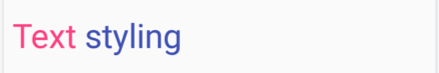
\includegraphics[width=0.5\textwidth,keepaspectratio]{images/span}
    \end{center}
\end{frame}

\begin{frame}[fragile]
    \frametitle{Стилизация строк с использованием Spans}
    \begin{minted}{java}
        CharSequence format = "{span} styling"
        SpannableString spannable = new SpannableString("Text");
        spannable.setSpan(ForegroundColorSpan(Color.PINK),
            0, 4, Spannable.SPAN_EXCLUSIVE_EXCLUSIVE);
        CharSequence fullText = Phrase.from(format)
            .put("span", spannable)
            .format()
        spanTextView.setText(fullText);
    \end{minted}
\end{frame}
\begin{frame}[fragile]
    \frametitle{HTML как альтернатива}
    \begin{minted}{xml}
        <string name="html_example"><b>Text</b> styling</string>
    \end{minted}
    \begin{minted}{java}
        spanTextView.setText(R.string.html_example);
        // or, but note getText usage instead of getString
        spanTextView.setText(getText(R.string.html_example));
    \end{minted}
\end{frame}

\begin{frame}[fragile]
    \frametitle{Фиксированный размер UI-элементов}
    \begin{minted}{xml}
        <!-- Bad -->
        <Button
            android:layout_width="120dp"
            android:layout_height="48dp"
            android:text="@string/do_the_thing_label"/>
        <!-- Good -->
        <Button
            android:layout_width="wrap_content"
            android:layout_height="wrap_content"
            android:text="@string/do_the_thing_label"/>
        <!-- Even better -->
        <Button
            android:layout_width="wrap_content"
            android:layout_height="wrap_content"
            android:minWidth="120dp"
            android:minWHeight="48dp"
            android:text="@string/do_the_thing_label"/>
    \end{minted}
\end{frame}

\begin{frame}[fragile]
    \frametitle{Отсутствие поддержки RTL-локалей}
    \begin{minted}{xml}
        <!-- Bad -->
        <Button
            android:id="@+id/do_the_thing"
            android:layout_width="wrap_content"
            android:layout_height="wrap_content"
            android:layout_marginLeft="16dp"
            android:layout_marginRight="64dp"
            android:text="@string/do_the_thing_label"/>
    \end{minted}
    \begin{minted}{xml}
        <!-- Good -->
        <Button
            android:id="@+id/do_the_thing"
            android:layout_width="wrap_content"
            android:layout_height="wrap_content"
            android:layout_marginStart="16dp"
            android:layout_marginEnd="64dp"
            android:text="@string/do_the_thing_label"/>
    \end{minted}
\end{frame}

\begin{frame}
    \frametitle{Текст в изображениях}
    \begin{center}
        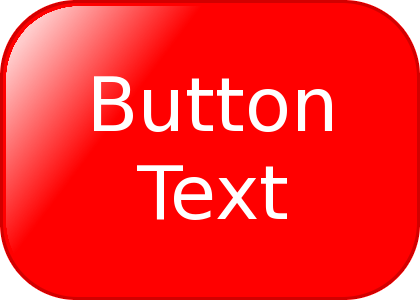
\includegraphics[width=0.3\textwidth,keepaspectratio]{images/button}
    \end{center}
    \begin{itemize}
        \item Заменить на стандартный виджет
        \item Заменить на кастомный виджет
        \item Разбить фон и текст и заменить текст на стандартный виджет
        \item Разбить фон и текст и создать копии текста для разных языков
        \item Создать копии изображения для разных языков
    \end{itemize}
\end{frame}

\begin{frame}
    \frametitle{Локализация с использованием ресурсов}
    \begin{center}
        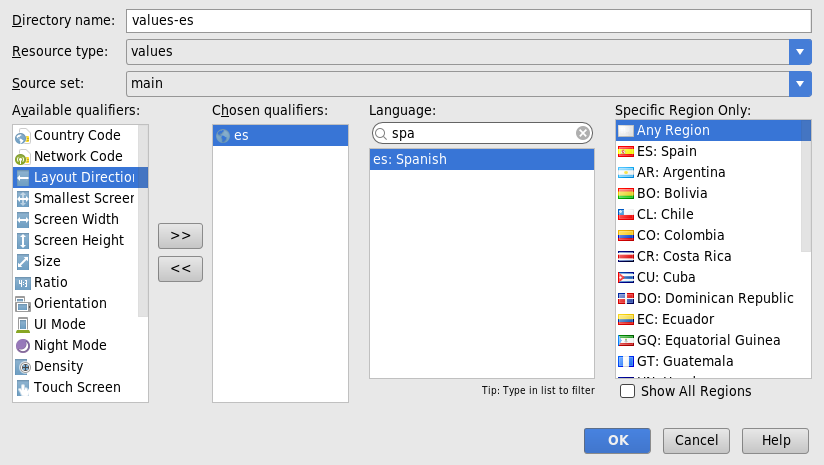
\includegraphics[width=0.7\textwidth,keepaspectratio]{images/resources}
    \end{center}
    \begin{itemize}
        \item UI - \texttt{res/layout/}
        \item Строки - \texttt{res/values/strings.xml}
        \item Изображения \texttt{res/drawable/}
        \item и т. д.
    \end{itemize}
\end{frame}

\begin{frame}
    \frametitle{Локализация с использованием ресурсов}
    \begin{itemize}
        \item Должен быть набор дефолтных ресурсов
        \item Ресурсы со спецификатором локали имеют приоритет над другими ресурсами
            (\texttt{res/drawable-small-land-stylus/ vs. res/drawable-es/})
    \end{itemize}
\end{frame}

\begin{frame}
    \frametitle{Lint}
    \begin{itemize}
        \item \textbf{HardcodedText} - текст в layout-файлах
        \item \textbf{SetTextI18n} - текст в коде, конкатенация строк
        \item \textbf{MissingTranslation} - если строковый ресурс есть в
            дефолтных ресурсах, но отсутствует в ресурсах для конкретной
            локали. Если строка не подлежит переводу, то
            должна быть объявлена с флагом \texttt{translatable=false}
        \item \textbf{ExtraTranslation} - если строковый ресурс есть в ресурсах
			для конкретной локали, но нет в дефолтных.
        \item \textbf{ImpliedQuantity, PluralsCandidate}
    \end{itemize}
\end{frame}

\begin{frame}[fragile]
    \frametitle{Псевдолокализация}
    \begin{minted}{groovy}
        android {
            // ...

            buildTypes {
                debug {
                    pseudoLocalesEnabled true
                }
            }
        }
    \end{minted}
    \begin{itemize}
        \item \textbf{en-XA} - добавляет глифы и увеличивает длину строк
        \item \textbf{ar-XB} - переворачивает строки справо налево и устанавливает
            направление текста справо налево.
    \end{itemize}
\end{frame}

\begin{frame}
    \frametitle{Псевдолокализация}
    \begin{center}
        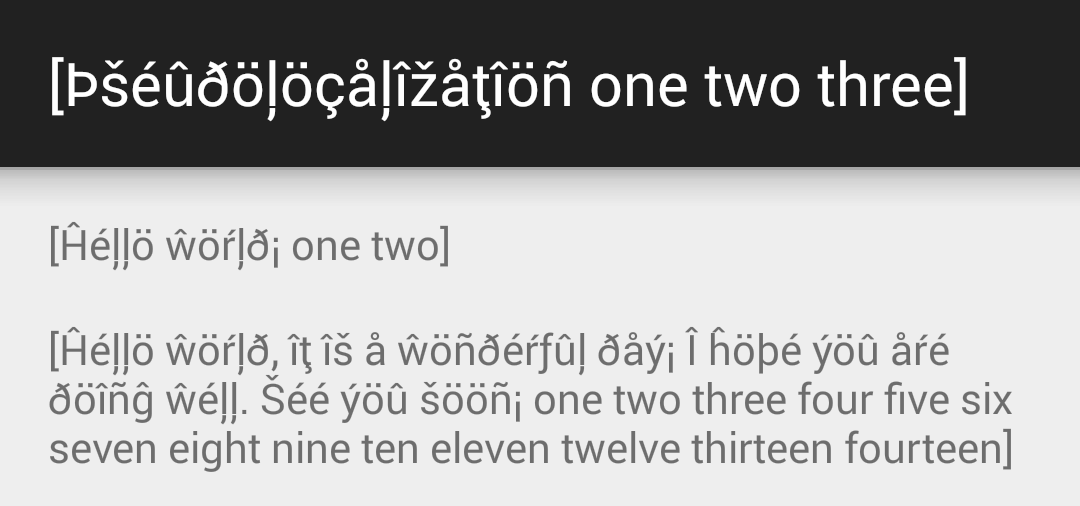
\includegraphics[width=0.7\textwidth,keepaspectratio]{images/pseudolocalization}
    \end{center}
\end{frame}

\begin{frame}
    \frametitle{Ссылки}
    \nocite{*}
    \RaggedRight
    \AtNextBibliography{\scriptsize}
    \printbibliography[heading=none]
\end{frame}

\begin{frame}
    \frametitle{Вопросы?}
\end{frame}

\end{document}
